% ======================================================================
%  Final presentation, CSC 591/791 / ECE 591 Deep Learning Beyond Accuracy
%  Compression vs. group robustness on Waterbirds
%  Every number here was computed from the repo's own CSVs.
% ======================================================================
\documentclass[aspectratio=169,10pt]{beamer}
\usepackage[T1]{fontenc}
\usepackage[default,semibold]{sourcesanspro}
\usepackage{tikz}
\usepackage{pgfplots}
\pgfplotsset{compat=1.18}
\usetikzlibrary{positioning,arrows.meta,calc,fit,backgrounds}
\usepackage{booktabs}
\usepackage{array}
\usepackage{amsmath}
\usepackage{graphicx}
\usepackage{qrcode}

% ---------------------------------------------------------------- palette
\definecolor{wolfred}{HTML}{CC0000}   % NC State Wolfpack Red
\definecolor{reynolds}{HTML}{990000}  % Reynolds Red
\definecolor{deepred}{HTML}{7A0000}   % darkest stop of the title gradient
\definecolor{midred}{HTML}{A80000}    % the gradient's middle
\definecolor{ink}{HTML}{1A1A1A}
\definecolor{slate}{HTML}{6E6E6E}
\definecolor{mist}{HTML}{F3F3F3}
\definecolor{ashe}{HTML}{DADADA}
\definecolor{teal}{HTML}{2E6E7E}      % the "with fix" series

% ---------------------------------------------------------------- theme
\usetheme{default}
\setbeamertemplate{navigation symbols}{}
\setbeamercolor{normal text}{fg=ink}
\setbeamercolor{structure}{fg=wolfred}
\setbeamerfont{frametitle}{size=\large,series=\bfseries}

% title band: title and subtitle stacked, never collide
\setbeamertemplate{frametitle}{%
  \nointerlineskip%
  \vskip0.55ex%
  \qrbadge%
  \hspace*{0.9em}%
  % Fixed height: the natural height varied with the title's descenders,
  % shifting the red rule by up to 2.8 mm from slide to slide.
  \begin{minipage}[t][9.8mm][t]{0.855\paperwidth}
    \raggedright
    {\color{wolfred}\usebeamerfont{frametitle}\insertframetitle}%
    \ifx\insertframesubtitle\@empty\else
      \par\vskip0.25ex
      {\color{slate}\footnotesize\insertframesubtitle}%
    \fi
  \end{minipage}%
  \par\vskip0.55ex%
  \hspace*{0.9em}{\color{wolfred}\rule{0.957\paperwidth}{1.1pt}}%
  \par\vskip0.85ex%
}

\setbeamertemplate{footline}{%
  \hbox{}\vskip-1.6ex%
  \hspace*{0.9em}{\color{ashe}\rule{0.957\paperwidth}{0.4pt}}\par\vskip0.4ex%
  \hspace*{0.9em}\raisebox{-0.35ex}{\brickred{2.4mm}}\hspace{0.7em}%
  {\color{slate}\fontsize{6.5}{8}\selectfont
    Compression vs. group robustness on Waterbirds}%
  \hfill{\color{wolfred}\fontsize{8}{9}\selectfont\bfseries\insertframenumber}%
  \hspace*{0.9em}\vskip0.55ex%
}

% ---------------------------------------------------------------- helpers
% Figure type, 3 pt larger than the \tiny / \scriptsize these replaced:
% at the back of a lecture hall the old sizes were not readable.
\newcommand{\figS}{\fontsize{8}{9.6}\selectfont}
\newcommand{\figM}{\fontsize{10}{12}\selectfont}
\newcommand{\hl}[1]{{\color{wolfred}\bfseries\boldmath #1}}
\newcommand{\hlt}[1]{{\color{teal}\bfseries\boldmath #1}}
\newcommand{\redbar}{{\color{wolfred}\rule{2.0em}{2.4pt}}}

% soft grey panel
\newcommand{\panel}[2][0.95]{%
  \begin{tikzpicture}
  \node[fill=mist,rounded corners=2pt,inner sep=7pt,text width=#1\textwidth,
        align=left,font=\small]{#2};
  \end{tikzpicture}}
% red-outlined callout
\newcommand{\callout}[2][0.95]{%
  \begin{tikzpicture}
  \node[draw=wolfred,line width=1pt,fill=wolfred!5,rounded corners=2pt,
        inner sep=8pt,text width=#1\textwidth,align=left,font=\small]{#2};
  \end{tikzpicture}}

\renewcommand{\arraystretch}{1.18}

% Official NC State brick logos, from brand.ncsu.edu/downloads.
% brickred  = red brick, white type   -> for white backgrounds
% brickwhite = white brick, red type  -> for red backgrounds
\newcommand{\brickred}[1]{
\includegraphics[height=#1]{assets/ncstate-brick-4x1-red-max.png}}
\newcommand{\brickwhite}[1]{
\includegraphics[height=#1]{assets/ncstate-brick-2x1-white-red-type-rgb-max.png}}

% The report, published at github.com/FirefoxSRV/waterbirds and served by
% GitHub Pages as application/pdf, so a phone opens it in its own viewer
% instead of downloading it.
\newcommand{\reporturl}{https://firefoxsrv.github.io/waterbirds/UNDERSTAND.pdf}
% Built once into a box: \qrcode uses deep grouping, and running it inside
% the frametitle template on every slide overruns TeX's 255 grouping levels.
% The code, same account. Private at the time of writing: this link only
% resolves for the class once the repository is made public.
\newcommand{\repourl}{https://github.com/FirefoxSRV/compression-group-robustness}
\newsavebox{\qrbox}
\newsavebox{\qrreport}
\newsavebox{\qrrepo}
\AtBeginDocument{%
  \sbox{\qrbox}{\qrcode[height=7.5mm,level=M]{\reporturl}}%
  \sbox{\qrreport}{\qrcode[height=19mm,level=M]{\reporturl}}%
  \sbox{\qrrepo}{\qrcode[height=19mm,level=M]{\repourl}}}
% Absolutely placed, so it never takes part in a frame's layout. The white
% fill is invisible on a white slide and gives the code its quiet zone on red.
\newcommand{\qrbadge}{%
  \begin{tikzpicture}[remember picture,overlay]
    \node[anchor=north east,fill=white,rounded corners=1.5pt,inner sep=2pt]
      at ($(current page.north east)+(-0.46,-0.24)$) {\usebox{\qrbox}};
  \end{tikzpicture}}

\pgfplotsset{
  slide/.style={
    font=\figM,
    axis line style={slate,line width=0.5pt},
    tick label style={slate},
    label style={ink,font=\figM},
    grid=major,
    major grid style={ashe,line width=0.4pt},
    tick align=outside, tick pos=left,
    legend style={draw=none,fill=none,font=\figM},
  }
}

% ======================================================================
\begin{document}

% ------------------------------------------------------------ 1. TITLE
{%
\setbeamertemplate{footline}{}
\begin{frame}[plain]
\begin{tikzpicture}[remember picture,overlay]
  % deep red to Wolfpack red, angled. The dark stop keeps it off orange.
  \shade[shading angle=25, top color=wolfred, bottom color=deepred]
    (current page.south west) rectangle (current page.north east);
  % a second blend on a crossing axis: depth without a visible edge
  \shade[shading angle=115, top color=deepred, bottom color=midred,
         opacity=0.38]
    (current page.south west) rectangle (current page.north east);

  % white brick, top left
  \node[anchor=north west] at ($(current page.north west)+(0.88,-0.62)$)
    {\brickwhite{8.2mm}};
  \qrbadge

  \node[anchor=north west,text width=0.78\paperwidth,align=left]
    at ($(current page.north west)+(0.88,-2.05)$) {%
    \color{white}\fontsize{22}{26}\selectfont\bfseries\raggedright
    Does model compression\\quietly break group robustness?\par
    \vskip0.6em
    {\fontsize{10.5}{13.2}\selectfont\mdseries\raggedright
    We compress a ViT that learned a background shortcut and ask who pays.
    Then we apply a published fix and ask whether it survives.\par}
  };

  % white panel: the one bright block on a red page
  \node[anchor=south west,fill=white,rounded corners=3pt,inner sep=9pt,
        text width=0.735\paperwidth,align=left]
    at ($(current page.south west)+(0.88,0.55)$) {%
    {\color{wolfred}\rule{1.8em}{2.2pt}}\par\vskip0.55em
    % the unity id sits off its name by a visible gap, not a word space
    {\color{ink}\footnotesize\textbf{Anusha Upadhyay}\hspace{0.45em}%
      {\scriptsize\color{slate}aupadhy6}\quad
      \textbf{Shreyas Visweshwaran}\hspace{0.45em}%
      {\scriptsize\color{slate}sviswes}\quad
      \textbf{Swasti Sadanand}\hspace{0.45em}%
      {\scriptsize\color{slate}ssadana}}\par
    \vskip0.45em
    {\color{slate}\scriptsize CSC 591/791, ECE 591: Deep Learning Beyond
    Accuracy}
  };
\end{tikzpicture}
\end{frame}
}

% ------------------------------------------------------------ 2. INDEX
% one row per part. The page numbers are checked against the built PDF.
\newcommand{\agendarow}[4]{%
  \noindent
  \begin{minipage}[c]{0.085\textwidth}
    \tikz\node[fill=wolfred,rounded corners=2pt,text=white,
               font=\bfseries\large,minimum width=0.82cm,
               minimum height=0.82cm,inner sep=0pt]{#1};
  \end{minipage}%
  \begin{minipage}[c]{0.755\textwidth}
    {\small\bfseries\color{ink}#2}\par\vskip0.12em
    {\scriptsize\color{slate}#3}
  \end{minipage}%
  \begin{minipage}[c]{0.16\textwidth}
    \raggedleft{\scriptsize\bfseries\color{wolfred}#4}
  \end{minipage}%
  \par}
\newcommand{\agendarule}{\vskip0.55em
  {\color{ashe}\rule{\textwidth}{0.4pt}}\par\vskip0.55em}

\begin{frame}{Where this talk goes}
{four parts, thirteen minutes}

\agendarow{1}{Setup: the trap, and the ruler}
  {The shortcut, why one average lies, the frozen scope, the 29-setting
   grid.}%
  {pages 3 to 8}
\agendarule
\agendarow{2}{Phase 1: compress a model that is already biased}
  {What 29 settings do to the average, the worst group and the gap.}%
  {pages 9 to 13}
\agendarule
\agendarow{3}{Phase 2: fix the robustness first, then compress}
  {The published fix reproduced, and how much survives compression.}%
  {pages 14 to 18}
\agendarule
\agendarow{4}{Closing: what it cost, and what it taught us}
  {Challenges, contributions, and what we would want remembered.}%
  {pages 19 to 21}

\vskip0.75em
% a narrower band, centred: the full width left a lot of empty grey
{\centering\panel[0.74]{Every number is from our own runs, \hl{3 seeds} in
both phases.}\par}
\end{frame}

% ------------------------------------------------------------ 2. HOOK
\begin{frame}{The question, and the answer}
{Phase 1 headline, mean of 3 seeds}
\begin{columns}[T,onlytextwidth]
\begin{column}{0.47\textwidth}
\small
Everybody compresses before shipping, and reports one number: average
accuracy.
\vskip0.6em
We pruned \hl{30\% of the weights} from a fine-tuned ViT-S/16 and read both.
\vskip0.8em
\panel[0.93]{%
  \textbf{\small Average accuracy} \hfill {\small $98.3 \rightarrow 97.8$}\par
  \vskip0.2em{\color{slate}a 0.5 point drop. Looks free.}\par
  \vskip0.6em
  \textbf{\small\color{wolfred}Worst-group accuracy} \hfill
    {\small\color{wolfred}$73.3 \rightarrow 58.4$}\par
  \vskip0.2em{\color{slate}a 14.9 point drop. Same operation.}}
\end{column}
\begin{column}{0.49\textwidth}
\centering
\vskip0.6em
{\color{wolfred}\fontsize{44}{46}\selectfont\bfseries 29\,$\times$}\par
\vskip0.4em
{\small\color{slate}worse for the weakest group\\than the average admits}
\vskip1.1em
{\color{ashe}\rule{0.75\textwidth}{0.6pt}}
\vskip1.0em
\callout[0.9]{%
Sharper still: delete \textbf{6 of 72 attention heads}, 2.8\% of the scope,
and the average loses 1.7 while the worst group loses \hl{18.2}.}

\end{column}
\end{columns}
\end{frame}

% ------------------------------------------------------------ 3. DATASET
\begin{frame}{Waterbirds: a dataset built to be a trap}
{birds cut out and pasted onto controlled backgrounds}
\begin{columns}[T,onlytextwidth]
\begin{column}{0.46\textwidth}
\centering
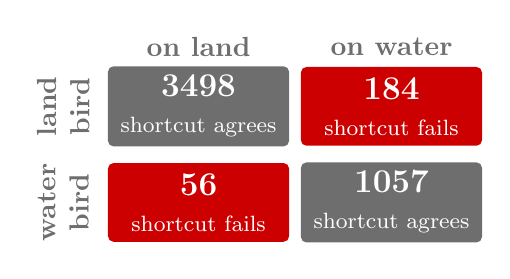
\begin{tikzpicture}[font=\figM,
  box/.style={minimum width=2.3cm,minimum height=1.0cm,align=center,
              rounded corners=2pt,text=white}]
  \node[font=\figM\bfseries,text=slate] at (1.2,1.06) {on land};
  \node[font=\figM\bfseries,text=slate] at (3.65,1.06) {on water};
  % Set on two lines: rotated, "water bird" is 1.6 cm long against a row
  % pitch of 1.22 cm, so the two labels collided.
  \node[rotate=90,font=\figM\bfseries,text=slate,align=center] at (-0.52,0.3)
       {land\\bird};
  \node[rotate=90,font=\figM\bfseries,text=slate,align=center] at (-0.52,-0.92)
       {water\\bird};
  \node[box,fill=slate]   at (1.2,0.3)   {\fontsize{13}{13}\selectfont\bfseries 3498\\[1pt]
       {\figS shortcut agrees}};
  \node[box,fill=wolfred] at (3.65,0.3)  {\fontsize{13}{13}\selectfont\bfseries 184\\[1pt]
       {\figS shortcut fails}};
  \node[box,fill=wolfred] at (1.2,-0.92) {\fontsize{13}{13}\selectfont\bfseries 56\\[1pt]
       {\figS shortcut fails}};
  \node[box,fill=slate]   at (3.65,-0.92){\fontsize{13}{13}\selectfont\bfseries 1057\\[1pt]
       {\figS shortcut agrees}};
\end{tikzpicture}
\par\vskip0.35em
{\footnotesize\color{slate}Training images per group. The two grey boxes
are 95\% of the data.}
\par\vskip0.65em
{\color{wolfred}\small\textbf{group}$\;=\;2y + \text{background}$}

\end{column}
\begin{column}{0.50\textwidth}
\small
\redbar\par\vskip0.6em
\textbf{The shortcut.} ``Is the background wet?'' is right 95\% of the time
and far easier to learn than bird anatomy. Plain training never punishes it.
\vskip0.7em
\textbf{Four groups}, bird crossed with background. Two agree with the
shortcut, two fight it. \hl{The weakest has 56 training images}.
\vskip0.9em
\panel[0.94]{\textbf{We train it badly on purpose.} No group labels, no
reweighting, no GroupDRO. The model is \emph{supposed} to learn the shortcut:
that is the experiment, not a mistake.}
\end{column}
\end{columns}
\end{frame}

% ------------------------------------------------------------ 4. METRICS
\begin{frame}{What we measure, and why the average lies}
{our fine-tuned ViT-S/16, before any compression}
\begin{columns}[T,onlytextwidth]
% The left column carries both figures, so it takes the wider share: the
% count cells were unreadable from the back at the old 0.50 split.
\begin{column}{0.56\textwidth}
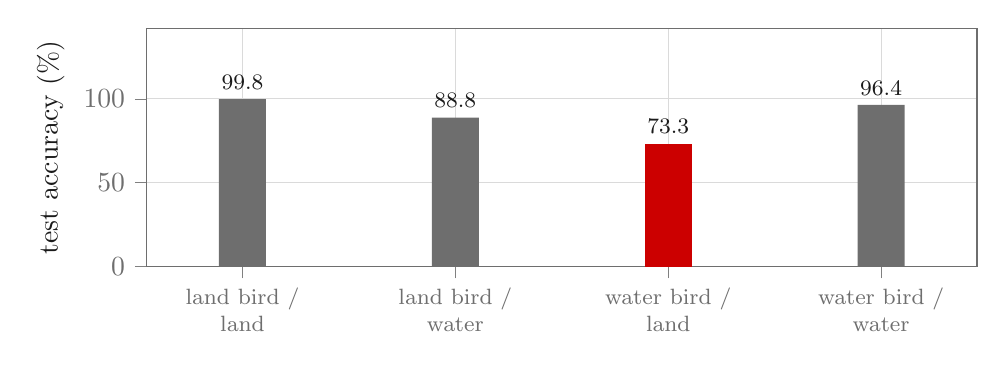
\begin{tikzpicture}
\begin{axis}[slide, width=\linewidth, height=0.46\linewidth,
  % 0.355 of a wider column is the same plot height as before: the
  % extra width went to the bars, not to vertical room the slide lacks.
  ybar, bar width=17pt, height=0.38\linewidth,
  % headroom is in DATA units: at this height 112 leaves less room above a
  % 99.8 bar than the "nodes near coords" label is tall, so it breaks the rule.
  ymin=0, ymax=142, ytick={0,50,100},
  ylabel={test accuracy (\%)},
  symbolic x coords={g0,g1,g2,g3}, xtick={g0,g1,g2,g3},
  xticklabels={{land bird /\\land},{land bird /\\water},{water bird /\\land},{water bird /\\water}},
  xticklabel style={align=center,font=\figS},
  nodes near coords, nodes near coords style={font=\figS,color=ink},
  every node near coord/.append style={/pgf/number format/fixed,
     /pgf/number format/precision=1},
  enlarge x limits=0.15,
]
% both series sit in their own category slot: without bar shift=0pt
% pgfplots offsets them and the x labels stop matching their bars.
\addplot[fill=slate,draw=none,bar shift=0pt]
  coordinates {(g0,99.8)(g1,88.8)(g3,96.4)};
\addplot[fill=wolfred,draw=none,bar shift=0pt]
  coordinates {(g2,73.3)};
\end{axis}
\end{tikzpicture}
\par\vskip0.15em
{\footnotesize\color{slate}A 26 point spread, best to worst group.}
\par\vskip0.35em
% Counts set at \figM in cells half again as large: these four numbers are
% the whole argument of the slide and were the smallest type on it.
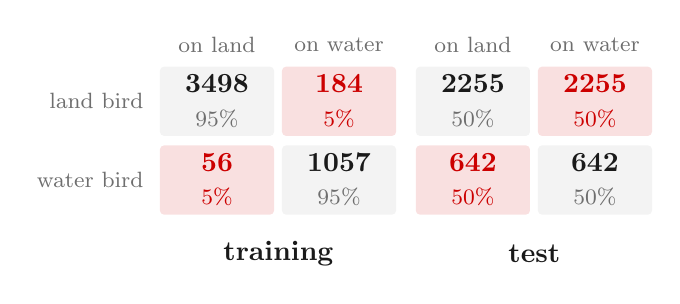
\begin{tikzpicture}[font=\figM,
  c/.style={minimum width=1.45cm,minimum height=0.88cm,align=center,
            inner sep=0pt,rounded corners=1.5pt},
  ok/.style={c,fill=mist,text=ink},
  no/.style={c,fill=wolfred!12,text=wolfred},
  hd/.style={text=slate,font=\figS},
  rl/.style={text=slate,font=\figS,anchor=east}]
  % column headers
  \node[hd] at (0.78,0.72) {on land};  \node[hd] at (2.33,0.72) {on water};
  \node[hd] at (4.03,0.72) {on land};  \node[hd] at (5.58,0.72) {on water};
  % row labels, shared by both matrices
  \node[rl] at (-0.03,0.0)   {land bird};
  \node[rl] at (-0.03,-1.00) {water bird};
  % training
  \node[ok] at (0.78,0.0)   {\textbf{3498}\\{\figS\color{slate}95\%}};
  \node[no] at (2.33,0.0)   {\textbf{184}\\{\figS 5\%}};
  \node[no] at (0.78,-1.00) {\textbf{56}\\{\figS 5\%}};
  \node[ok] at (2.33,-1.00) {\textbf{1057}\\{\figS\color{slate}95\%}};
  % test
  \node[ok] at (4.03,0.0)   {\textbf{2255}\\{\figS\color{slate}50\%}};
  \node[no] at (5.58,0.0)   {\textbf{2255}\\{\figS 50\%}};
  \node[no] at (4.03,-1.00) {\textbf{642}\\{\figS 50\%}};
  \node[ok] at (5.58,-1.00) {\textbf{642}\\{\figS\color{slate}50\%}};
  % captions
  \node[text=ink,font=\figM\bfseries] at (1.56,-1.94) {training};
  \node[text=ink,font=\figM\bfseries] at (4.81,-1.94) {test};
\end{tikzpicture}
\end{column}
\begin{column}{0.41\textwidth}
\small
\begin{tabular}{@{}l r l@{}}
\toprule
\textbf{number} & \textbf{ours} & \textbf{what it is}\\
\midrule
plain average    & 91.7\% & straight test mean\\
adjusted average & 98.3\% & reweighted to train\\
\textbf{\color{wolfred}worst group}
 & \textbf{\color{wolfred}73.3\%} & the weakest group\\
\bottomrule
\end{tabular}
\vskip0.6em
\panel[0.95]{\textbf{Why two averages.} Both splits are 77\% land birds, so
classes are not what differs; the \emph{background} is, 95/5 in training
against 50/50 in test. The red groups are \hl{5\% of training, 50\% of test},
so a plain test mean over-weights them tenfold.}
\vskip0.5em
{\footnotesize \hl{Worst group is the honest number.}}
\par\vskip0.45em
{\footnotesize\color{slate}Red cells are the groups that fight the shortcut.}
\end{column}
\end{columns}
\end{frame}

% ------------------------------------------------------------ 5. ARCHITECTURE
\begin{frame}{Project structure, end to end}
{Phase 1 trains once and compresses 29 ways. Phase 2 adds a step in front.}
% Spans the full paper width, not \textwidth: the stage boxes were too
% small to read from the back of the room. \makebox keeps TeX quiet about
% the overhang into the side margins.
\makebox[\textwidth]{%
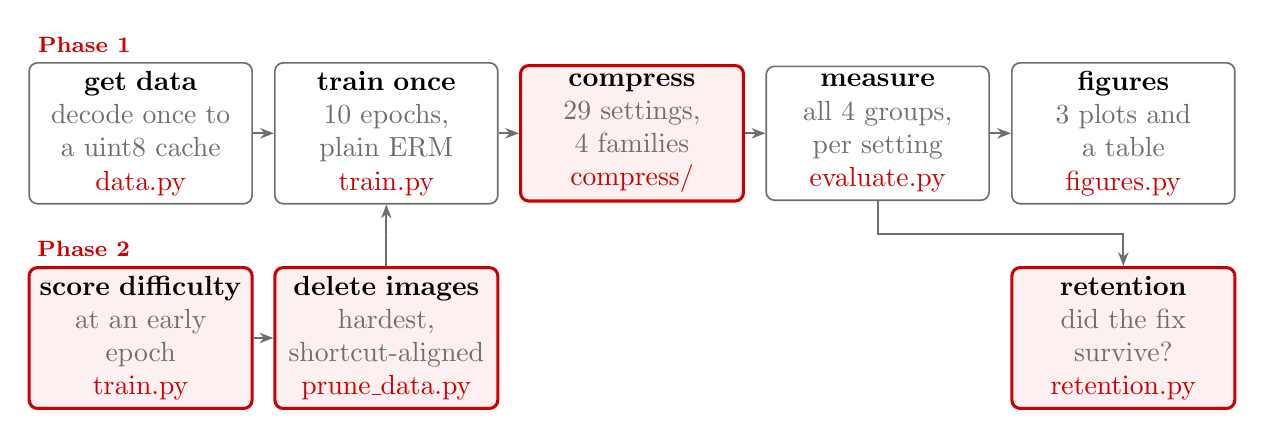
\begin{tikzpicture}[font=\figM,
  stage/.style={draw=slate,line width=0.6pt,fill=white,rounded corners=3pt,
                minimum height=1.32cm,text width=2.62cm,align=center,inner sep=3pt},
  red/.style={draw=wolfred,line width=1.1pt,fill=wolfred!6},
  ar/.style={-{Stealth[length=5pt]},slate,line width=0.7pt}]

% phase 1 row, explicit coordinates
\node[stage]     (data)  at (0,0)    {\textbf{get data}\\{\color{slate}decode once
     to a uint8 cache}\\{\color{wolfred}data.py}};
\node[stage]     (train) at (3.12,0) {\textbf{train once}\\{\color{slate}10 epochs,
     plain ERM}\\{\color{wolfred}train.py}};
\node[stage,red] (comp)  at (6.24,0)  {\textbf{compress}\\{\color{slate}29 settings,
     4 families}\\{\color{wolfred}compress/}};
\node[stage]     (eval)  at (9.36,0) {\textbf{measure}\\{\color{slate}all 4 groups,
     per setting}\\{\color{wolfred}evaluate.py}};
\node[stage]     (fig)   at (12.48,0) {\textbf{figures}\\{\color{slate}3 plots and
     a table}\\{\color{wolfred}figures.py}};
\draw[ar](data)--(train); \draw[ar](train)--(comp);
\draw[ar](comp)--(eval);  \draw[ar](eval)--(fig);

% phase 2 row
\node[stage,red] (score) at (0,-2.6)    {\textbf{score difficulty}\\{\color{slate}at
     an early epoch}\\{\color{wolfred}train.py}};
\node[stage,red] (prune) at (3.12,-2.6) {\textbf{delete images}\\{\color{slate}hardest,
     shortcut-aligned}\\{\color{wolfred}prune\_data.py}};
\node[stage,red] (ret)   at (12.48,-2.6) {\textbf{retention}\\{\color{slate}did the
     fix survive?}\\{\color{wolfred}retention.py}};
\draw[ar](score)--(prune);
% The turn is taken at the midpoint between the two rows, computed from the
% nodes themselves: a fixed offset put the elbow on the retention box's lid.
\draw[ar](prune.north) |- ($(prune.north)!0.5!(train.south)$) -| (train.south);
\draw[ar](eval.south)  |- ($(eval.south)!0.5!(ret.north)$)   -| (ret.north);

% Row tags sit ABOVE the first box of each row. Anchored east in the left
% margin they used to eat the horizontal room the boxes now need.
\node[font=\figS,text=wolfred,anchor=south west] at (data.north west)
  {\textbf{Phase 1}};
\node[font=\figS,text=wolfred,anchor=south west] at (score.north west)
  {\textbf{Phase 2}};
\end{tikzpicture}}
\vskip0.45em
\begin{columns}[T,onlytextwidth]
\begin{column}{0.48\textwidth}
\callout[0.95]{\textbf{No retraining after compression.} Fine-tuning would
re-learn the shortcut.}
\end{column}
\begin{column}{0.48\textwidth}
\panel[0.95]{\textbf{Scale.} 11,788 images, 29 settings, 3 seeds, 87 Phase 1
and 261 Phase 2 measurements, 9 hours on an M2 laptop.}
\end{column}
\end{columns}
\end{frame}

% ------------------------------------------------------------ 6. SCOPE
\begin{frame}{One frozen scope, four compression families}
{the design decision that makes the four numbers comparable}
% The block diagram now spans the full width instead of sharing a 0.43
% column: at the old size the box labels were unreadable from the back.
\centering
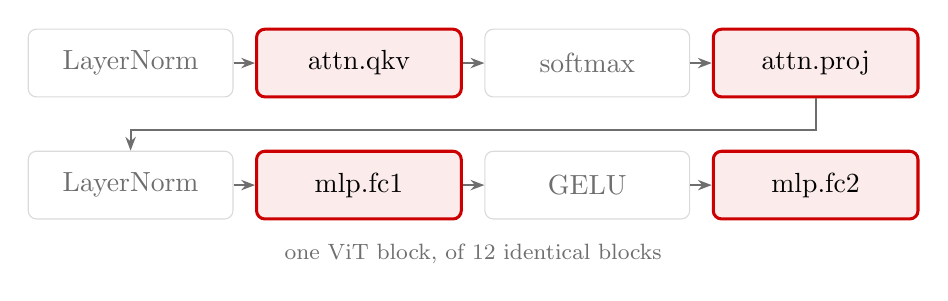
\begin{tikzpicture}[font=\figM,
  m/.style={draw=wolfred,line width=1.1pt,fill=wolfred!8,rounded corners=3pt,
            minimum width=2.6cm,minimum height=0.86cm,align=center,inner sep=2pt},
  o/.style={draw=ashe,fill=white,rounded corners=3pt,text=slate,
            minimum width=2.6cm,minimum height=0.86cm,align=center,inner sep=2pt},
  ar/.style={-{Stealth[length=5pt]},slate,line width=0.7pt}]
  \node[o] (ln1) at (0,0)   {LayerNorm};
  \node[m] (qkv) at (2.9,0) {attn.qkv};
  \node[o] (sm)  at (5.8,0) {softmax};
  \node[m] (pr)  at (8.7,0) {attn.proj};
  \node[o] (ln2) at (0,-1.55)   {LayerNorm};
  \node[m] (fc1) at (2.9,-1.55) {mlp.fc1};
  \node[o] (ge)  at (5.8,-1.55) {GELU};
  \node[m] (fc2) at (8.7,-1.55) {mlp.fc2};
  \draw[ar](ln1)--(qkv); \draw[ar](qkv)--(sm); \draw[ar](sm)--(pr);
  \draw[ar](ln2)--(fc1); \draw[ar](fc1)--(ge); \draw[ar](ge)--(fc2);
  \draw[ar](pr.south) -- ++(0,-0.4) -| (ln2.north);
  \node[text=slate,align=center,font=\figS] at (4.35,-2.42)
    {one ViT block, of 12 identical blocks};
\end{tikzpicture}
\par\vskip0.1em
\begin{columns}[T,onlytextwidth]
\begin{column}{0.44\textwidth}
\panel[0.97]{\centering\textbf{The scope, and what each matrix is for}%
\par\vskip0.25em
{\figS\begin{tabular}{@{}l@{\ \ }l@{}}
\textbf{\color{wolfred}attn.qkv}  & query, key, value per patch\\
\textbf{\color{wolfred}attn.proj} & mixes the 6 heads into one\\
\textbf{\color{wolfred}mlp.fc1}   & widens, 384 to 1536\\
\textbf{\color{wolfred}mlp.fc2}   & narrows back, 1536 to 384\\
\end{tabular}}\par\vskip0.25em
12 blocks $\times$ 4 matrices $=$ \hl{21,233,664 weights}, and nothing
else: no \mbox{embedding}, LayerNorm, bias or head.}
\end{column}
\begin{column}{0.52\textwidth}
\small
\begin{tabular}{@{}l l l@{}}
\toprule
\textbf{family} & \textbf{what it does} & \textbf{kind}\\
\midrule
magnitude & zero the smallest weights & unstructured\\
heads     & delete whole heads        & structured\\
ffn       & delete whole MLP neurons  & structured\\
quantize  & 8, 6, 4 or 3 bits         & precision\\
\bottomrule
\end{tabular}
\vskip0.3em
{\footnotesize $7+7+7+8 = $ \hl{29 settings}, all four groups re-measured.}

\end{column}
\end{columns}
\end{frame}

% ------------------------------------------------------------ 6b. THE SWEEP
% the grid itself: 7+7+7+8, and the knob-vs-sparsity distinction it exposes
\begin{frame}{The sweep: every setting we measured}
{29 per seed, 3 seeds, 87 measurements, all on the one frozen scope}
\centering
{\small\renewcommand{\arraystretch}{1.06}
\begin{tabular}{@{}l l c r@{}}
\toprule
\textbf{family} & \textbf{settings we ran} & \textbf{n} &
\textbf{weights actually zeroed}\\
\midrule
magnitude   & 0, 30, 50, 70, 80, 90, 95\% of weights      & 7 & 0 to 95.0\%\\
heads       & 0, 6, 12, 24, 36, 48, 60 of 72 heads        & 7 & 0 to 27.8\%\\
ffn         & 0, 30, 50, 70, 80, 90, 95\% of MLP neurons  & 7 & 0 to 63.3\%\\
quantize, per channel & 8, 6, 4, 3 bits per weight        & 4 & 1.4 to 48.9\%\\
quantize, per tensor  & 8, 6, 4, 3 bits per weight        & 4 & 4.8 to 90.3\%\\
\midrule
\multicolumn{2}{@{}l}{\textbf{per seed}} & \hl{29} &
  $\times$ 3 seeds $=$ \hl{87 rows}\\
\bottomrule
\end{tabular}}
\par\vskip0.5em
{\footnotesize\color{slate}Every row re-measures all four groups on the same
5794 test images.}
\vskip0.75em
\begin{columns}[T,onlytextwidth]
\begin{column}{0.47\textwidth}
\callout[0.95]{\textbf{The knob is not the sparsity.} 30\% of the MLP neurons
zeroes 20\% of the scope, since the MLP is two thirds of it. 6 of 72 heads
zeroes 2.8\%. \hl{Only magnitude's knob is the sparsity itself.}}
\end{column}
\begin{column}{0.47\textwidth}
{\small\textbf{Quantization deletes nothing.} Its percentage is how
many weights round to zero at that bit width: a symptom, not a target.
\vskip0.5em
\textbf{The zero level is a control:} every family re-measures the
uncompressed model first.}
\end{column}
\end{columns}
\end{frame}

% ------------------------------------------------------------ 7. RESULT 1
\begin{frame}{Phase 1: the gap opens, and the average hides it}
{magnitude pruning, mean of 3 seeds}
\begin{columns}[T,onlytextwidth]
\begin{column}{0.555\textwidth}
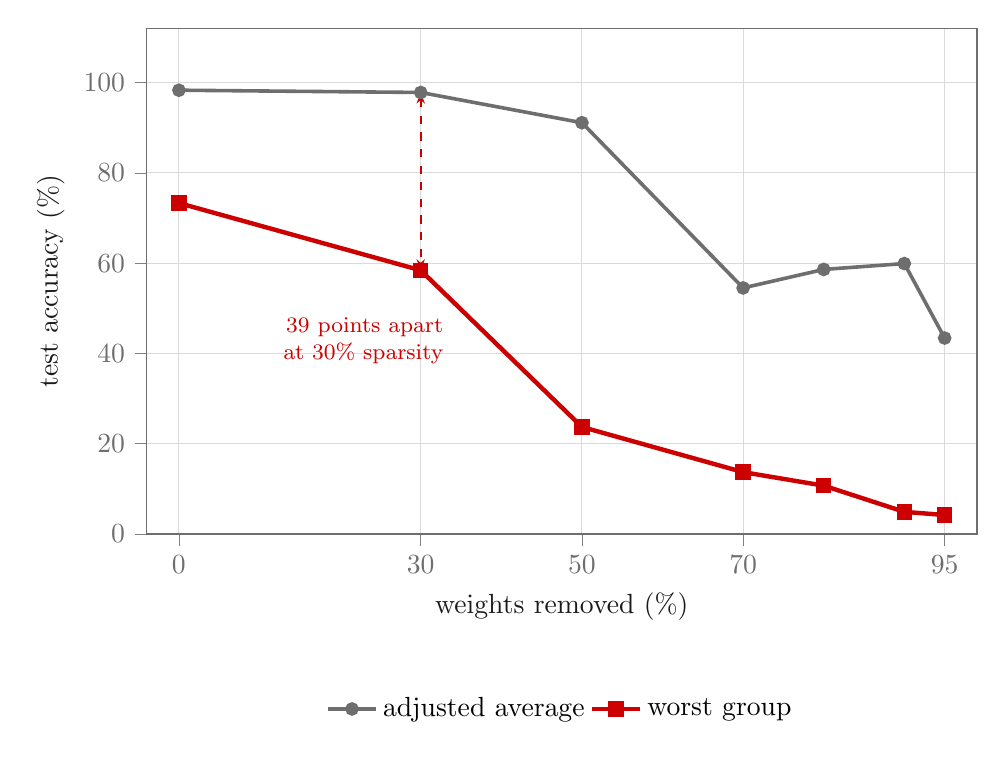
\begin{tikzpicture}
\begin{axis}[slide, width=\linewidth, height=0.66\linewidth,
  xlabel={weights removed (\%)}, ylabel={test accuracy (\%)},
  xmin=-4, xmax=99, ymin=0, ymax=112,
  xtick={0,30,50,70,95}, ytick={0,20,40,60,80,100},
  legend style={at={(0.5,-0.30)},anchor=north,legend columns=2,draw=none},
]
\addplot[slate,line width=1.3pt,mark=*,mark size=1.8pt] coordinates
  {(0,98.3)(30,97.8)(50,91.1)(70,54.5)(80,58.6)(90,59.9)(95,43.4)};
\addlegendentry{adjusted average}
\addplot[wolfred,line width=1.6pt,mark=square*,mark size=2.0pt] coordinates
  {(0,73.3)(30,58.4)(50,23.7)(70,13.7)(80,10.7)(90,4.9)(95,4.2)};
\addlegendentry{worst group}
\draw[wolfred,line width=0.8pt,dashed,{Stealth[length=4pt]}-{Stealth[length=4pt]}]
  (axis cs:30,97.8) -- (axis cs:30,58.4);
% Parked under the arrow's lower end, in the one corner no series crosses:
% at (36,82) it cut the adjusted-average line in half.
\node[font=\figS,color=wolfred,anchor=north east,align=right]
  at (axis cs:34,50) {39 points apart\\at 30\% sparsity};
\end{axis}
\end{tikzpicture}
\end{column}
\begin{column}{0.41\textwidth}
\small
\redbar\par\vskip0.6em
\textbf{The distance between the lines is the whole finding.} If they fell
together, compression would be fair to every group.
\vskip0.8em
\begin{tabular}{@{}l r r@{}}
\toprule
\textbf{removed} & \textbf{avg} & \textbf{worst}\\
\midrule
none & 98.3 & 73.3\\
30\% & 97.8 & \hl{58.4}\\
50\% & 91.1 & \hl{23.7}\\
70\% & 54.5 & 13.7\\
\bottomrule
\end{tabular}
\vskip0.9em
{\small At 30\% the average still reports a healthy model; the
weakest group has lost a fifth. At 50\% the average says 91 and the weakest
group sits at 24.}
\end{column}
\end{columns}
\end{frame}

% ------------------------------------------------------------ 8. RESULT 2
\begin{frame}{Phase 1: structured compression hurts most}
{5 of the 29 settings, one per family, mean of 3 seeds}
\centering
% tighter rows than the deck default: the excerpt note below needs the space
{\renewcommand{\arraystretch}{1.02}
\begin{tabular}{@{}l l r r r r@{}}
\toprule
\textbf{family} & \textbf{setting} & \textbf{sparsity} & \textbf{avg} &
\textbf{worst group} & \textbf{worst-group loss}\\
\midrule
\multicolumn{2}{@{}l}{\textit{no compression}} & 0.0\% & 98.3 & 73.3 & \\
\midrule
quantize, per channel & 6 bits          & 5.5\%  & 98.3 & 74.2 & \hlt{$+0.9$}\\
quantize, per tensor  & 6 bits          & 19.0\% & 97.7 & 68.1 & $-5.2$\\
magnitude             & 30\% of weights & 30.0\% & 97.8 & 58.4 & \hl{$-14.9$}\\
heads                 & 6 of 72 heads   & 2.8\%  & 96.6 & 55.1 & \hl{$-18.2$}\\
ffn                   & 30\% of neurons & 20.0\% & 81.3 & 22.6 & \hl{$-50.7$}\\
\bottomrule
\end{tabular}}
\par\vskip0.45em
% these 5 rows are a slice of the sweep; say so, and say where the rest are
{\footnotesize\color{slate}The lightest of each family. Full grid on page 8,
plotted on 11, split by group on 12.}
\vskip0.55em
\begin{columns}[T,onlytextwidth]
\begin{column}{0.47\textwidth}
\callout[0.95]{\textbf{6 heads} touch 2.8\% of the scope and cost
\textbf{18.2} points. Magnitude removes 30\% and costs 14.9. Ten times the
weights, less damage. \hl{Where you cut matters more than how much.}}
\end{column}
\begin{column}{0.47\textwidth}
{\small\textbf{The families are not interchangeable.} They differ in
\emph{where the model dies}: FFN by 30\%, magnitude at 50\%, per-channel
quantization only at 3 bits.
\vskip0.5em
\textbf{Granularity is not a detail.} At 4 bits, per-channel keeps 66.7\% and
per-tensor 8.0\%.}
\end{column}
\end{columns}
\end{frame}

% ------------------------------------------------------------ 9. RESULT 3
\begin{frame}{Phase 1: the same average, a very different worst group}
{all 29 settings, mean of 3 seeds}
\begin{columns}[T,onlytextwidth]
\begin{column}{0.53\textwidth}
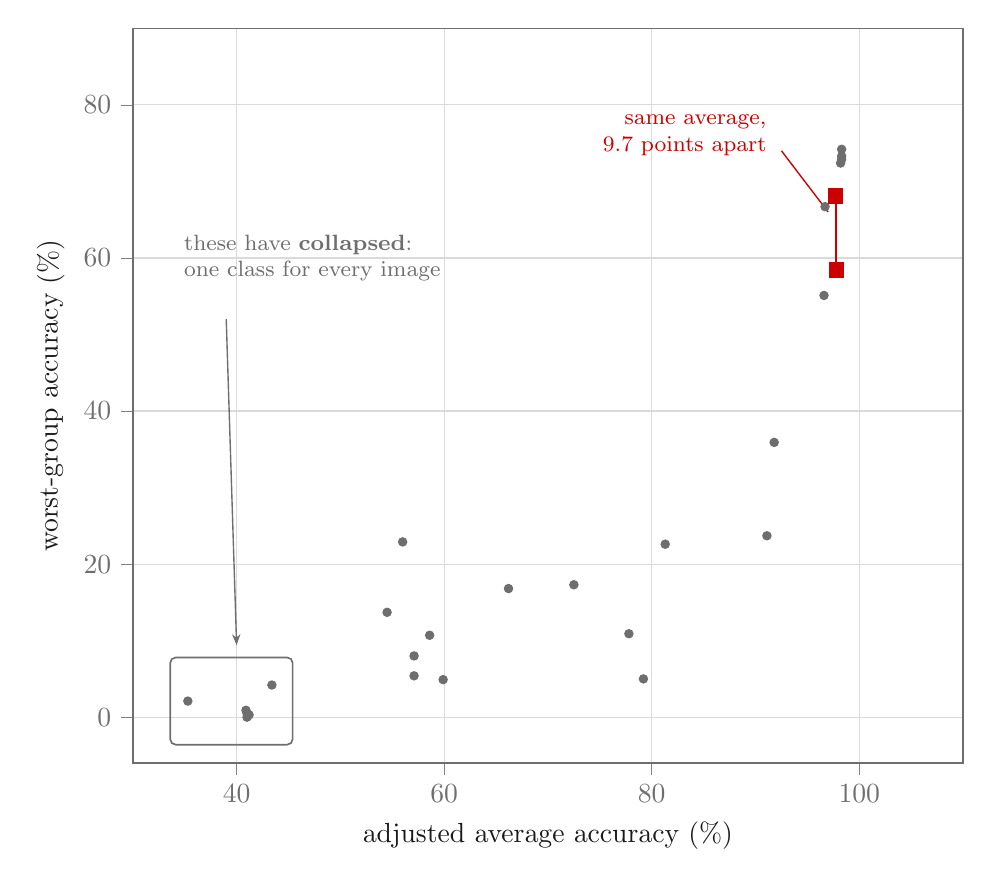
\begin{tikzpicture}
\begin{axis}[slide, width=\linewidth, height=0.90\linewidth,
  xlabel={adjusted average accuracy (\%)},
  ylabel={worst-group accuracy (\%)},
  xmin=30, xmax=110, ymin=-6, ymax=90,
  xtick={40,60,80,100}, ytick={0,20,40,60,80},
]
\addplot[only marks,mark=*,mark size=1.5pt,color=slate] coordinates {
 (35.3,2.1)(40.9,0.9)(41.0,0.5)(41.0,0.0)(41.2,0.3)(43.4,4.2)(54.5,13.7)
 (56.0,22.9)(57.1,5.4)(57.1,8.0)(58.6,10.7)(59.9,4.9)(66.2,16.8)(72.5,17.3)
 (77.8,10.9)(79.2,5.0)(81.3,22.6)(91.1,23.7)(91.8,35.9)(96.6,55.1)
 (96.7,66.7)(98.2,72.4)(98.3,74.2)(98.3,73.3)(98.3,72.9)};
\addplot[only marks,mark=square*,mark size=2.6pt,color=wolfred] coordinates
 {(97.8,58.4)(97.7,68.1)};
\draw[wolfred,line width=1pt] (axis cs:97.75,58.4) -- (axis cs:97.75,68.1);
\node[font=\figS,color=wolfred,anchor=east,align=right]
  at (axis cs:92,76) {same average,\\9.7 points apart};
\draw[wolfred,line width=0.5pt] (axis cs:92.5,74) -- (axis cs:97,66);
% these are collapsed models, not merely bad ones: say which it is
\node[font=\figS,color=slate,anchor=west,align=left]
  at (axis cs:34,60) {these have \textbf{collapsed}:\\
    one class for every image};
% ring the six collapsed settings, then point the label at the box
\draw[slate,line width=0.6pt,rounded corners=2pt]
  (axis cs:33.6,-3.6) rectangle (axis cs:45.4,7.8);
\draw[-{Stealth[length=4pt]},slate,line width=0.5pt]
  (axis cs:39,52) -- (axis cs:40,9.4);
\end{axis}
\end{tikzpicture}
\end{column}
\begin{column}{0.43\textwidth}
\small
\redbar\par\vskip0.6em
Each dot is one setting. \textbf{Pick a spot on the horizontal axis and look
up.} Dots stack: settings a standard evaluation calls equally good, at very
different worst-group accuracies.
\vskip0.8em
\begin{tabular}{@{}l r r@{}}
\toprule
\textbf{setting} & \textbf{avg} & \textbf{worst}\\
\midrule
6-bit, per tensor  & 97.7 & \hlt{68.1}\\
magnitude 30\%     & 97.8 & \hl{58.4}\\
\midrule
4-bit, per channel & 96.7 & \hlt{66.7}\\
6 heads of 72      & 96.6 & \hl{55.1}\\
\bottomrule
\end{tabular}
\vskip0.5em
{\footnotesize Two pairs, indistinguishable on average, 9.7 and 11.6 points
apart on the weakest group. \hl{That is what the average throws away.}}
\end{column}
\end{columns}
\end{frame}

% ------------------------------------------------------------ 10. RESULT 4
\begin{frame}{Phase 1: who actually pays}
{per-group accuracy, mean of 3 seeds}
\begin{columns}[T,onlytextwidth]
\begin{column}{0.555\textwidth}
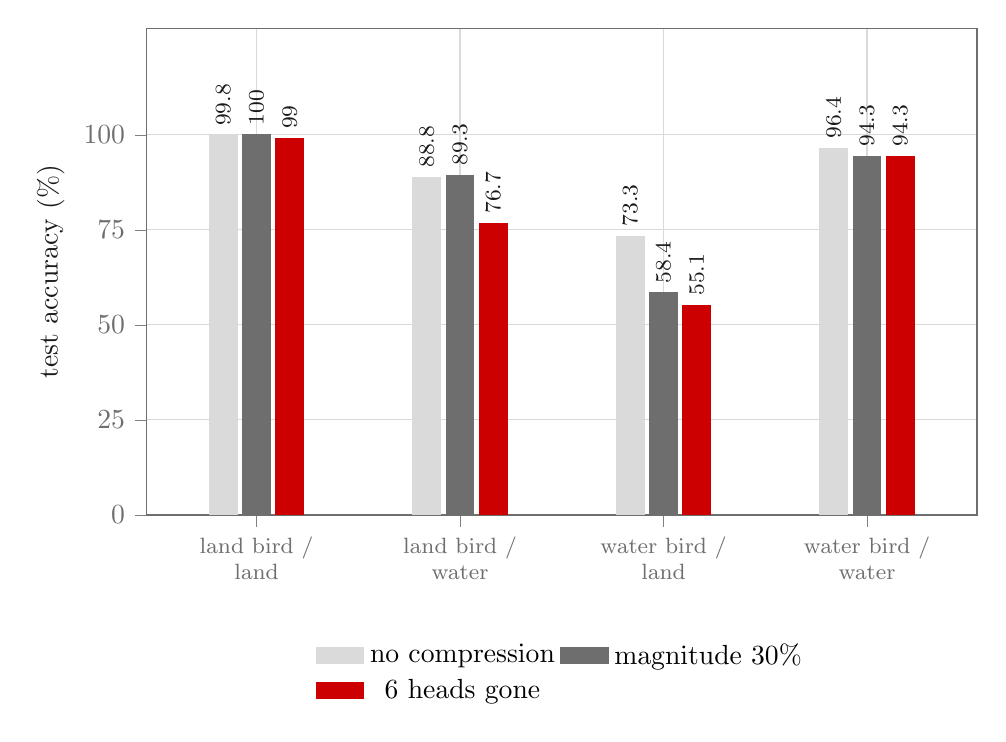
\begin{tikzpicture}
\begin{axis}[slide, width=\linewidth, height=0.64\linewidth,
  ybar, bar width=10pt,
  ymin=0, ymax=128, ytick={0,25,50,75,100},
  ylabel={test accuracy (\%)},
  symbolic x coords={g0,g1,g2,g3}, xtick=data,
  xticklabels={{land bird /\\land},{land bird /\\water},{water bird /\\land},{water bird /\\water}},
  xticklabel style={align=center,font=\figS},
  nodes near coords, nodes near coords style={font=\figS,color=ink,rotate=90,
     anchor=west},
  every node near coord/.append style={/pgf/number format/fixed,
     /pgf/number format/precision=1},
  enlarge x limits=0.18,
  legend style={at={(0.5,-0.24)},anchor=north,legend columns=2,draw=none},
]
\addplot[fill=ashe,draw=ashe,area legend] coordinates
  {(g0,99.8)(g1,88.8)(g2,73.3)(g3,96.4)};
\addlegendentry{no compression}
\addplot[fill=slate,draw=slate,area legend] coordinates
  {(g0,100.0)(g1,89.3)(g2,58.4)(g3,94.3)};
\addlegendentry{magnitude 30\%}
\addplot[fill=wolfred,draw=wolfred,area legend] coordinates
  {(g0,99.0)(g1,76.7)(g2,55.1)(g3,94.3)};
\addlegendentry{6 heads gone}
\end{axis}
\end{tikzpicture}
\end{column}
\begin{column}{0.41\textwidth}
\small
\redbar\par\vskip0.6em
\textbf{The damage is not spread out.} Under 30\% magnitude pruning three
groups move by under 2 points. The fourth, water birds on land, loses
\hl{14.9}.
\vskip0.8em
Those are the images where the shortcut is wrong: the only ones needing a
model that actually learned birds.
\vskip0.9em
\panel[0.95]{\textbf{The mechanism:} compression removes capacity, and the
first thing given up is whatever overrode the shortcut, which is cheap to
keep.}
\end{column}
\end{columns}
\end{frame}

% ------------------------------------------------------------ 11. COLLAPSE
\begin{frame}{A challenge worth naming: a collapsed model looks fair}
{21 of our 87 Phase 1 measurements are collapsed}
\begin{columns}[T,onlytextwidth]
\begin{column}{0.48\textwidth}
\small
Past about 70\% sparsity the gap starts \emph{shrinking} again. Robustness
returning? The opposite. A real row, magnitude at 80\%, seed 0:
\vskip0.4em
\centering
\begin{tabular}{@{}l r r r r r@{}}
\toprule
 & \textbf{g0} & \textbf{g1} & \textbf{g2} & \textbf{g3} & \textbf{adj avg}\\
\midrule
accuracy & 100\% & 100\% & 0\% & 0\% & \textbf{76.8\%}\\
\bottomrule
\end{tabular}
\par\vskip0.7em
\raggedright
That model answers ``land bird'' to \textbf{every image}: equally useless on
all four groups, so no disparity left to measure, yet a 76.8\% adjusted
average.
\end{column}
\begin{column}{0.48\textwidth}
\centering
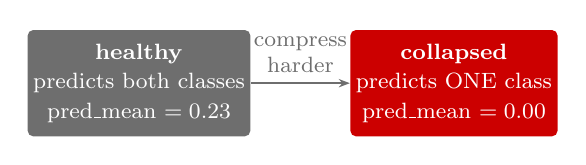
\begin{tikzpicture}[font=\figS,
  b/.style={rounded corners=2pt,minimum width=2.3cm,minimum height=1.35cm,
            align=center,text=white,inner sep=2pt},
  ar/.style={-{Stealth[length=4pt]},slate,line width=0.7pt}]
  \node[b,fill=slate] (h) at (0,0)
    {\textbf{healthy}\\[1pt]predicts both classes\\[1pt]pred\_mean $=0.23$};
  \node[b,fill=wolfred] (c) at (4.0,0)
    {\textbf{collapsed}\\[1pt]predicts ONE class\\[1pt]pred\_mean $=0.00$};
  \draw[ar](h)--node[above,font=\figS,text=slate,align=center]
    {compress\\harder}(c);
\end{tikzpicture}
\par\vskip0.9em
\callout[0.95]{\textbf{Our guard.} Every measurement records
\texttt{pred\_mean}, the average predicted class. Pinned near 0 or 1 means
collapsed, and those points are drawn hollow and excluded from every retention
number.\par\vskip0.4em
\hl{A small gap can mean ``fair'' or ``dead''.} Without this gate, the deep
end of every sweep reads as robustness recovering.}
\end{column}
\end{columns}
\end{frame}

% ------------------------------------------------------------ 12. PHASE 2 FIX
\begin{frame}{Phase 2: fix the robustness first, then compress}
{the fix is data pruning, from Varun Mulchandani and Jung-Eun Kim, ICLR 2025}
% Everything on this frame is set a point larger than the deck's default,
% and the left column carries two extra blocks: at \small it ended halfway
% down the slide while the right column ran on.
\begin{columns}[T,onlytextwidth]
\begin{column}{0.48\textwidth}
\normalsize
\panel[0.95]{\textbf{Why deleting data helps.} The model takes the
shortcut where the real bird features are hard. Delete those images and it
has less reason to learn the shortcut.}
\vskip0.6em
Difficulty of image $i$, scored after one epoch:
\vskip-0.5em
\[ d_i=\big\lVert\,p(x_i)-\mathrm{onehot}(y_i)\,\big\rVert_2 \]
\vskip-0.3em
With two classes this is exactly $\sqrt{2}\,(1-p_{\text{true}})$: the
distance from being certain and right.
\vskip0.6em
\panel[0.95]{ At the 50\% budget 4795 training images become 1170, and
every image in the two groups that fight the shortcut is kept.}
\end{column}
\begin{column}{0.48\textwidth}
\normalsize
\callout[0.96]{\textbf{The prune rule.} Take only images where the
background agrees with the bird, delete the hardest of those, never touch
the rest.\par\vskip0.4em
Groups are needed: the hardest images sit in the weak groups, so
\hl{deleting the globally hardest would delete what the fix protects}.}
\vskip0.55em
{\small The 50\% budget, on every seed:
\vskip0.35em
\begin{tabular}{@{}l r r@{}}
\toprule
\textbf{group} & \textbf{removed} & \textbf{of}\\
\midrule
g0 \ land on land   & 3097 & 3498\\
g3 \ water on water &  528 & 1057\\
g1 \ land on water  &    0 &  184\\
g2 \ water on land  &    0 &   56\\
\bottomrule
\end{tabular}}
\end{column}
\end{columns}
\end{frame}

% ------------------------------------------------------------ 13. FIX WORKS
\begin{frame}{Phase 2: the fix works, at every budget we tried}
{mean of 3 seeds, 3 deletion budgets, all 9 runs positive}
\begin{columns}[T,onlytextwidth]
\begin{column}{0.53\textwidth}
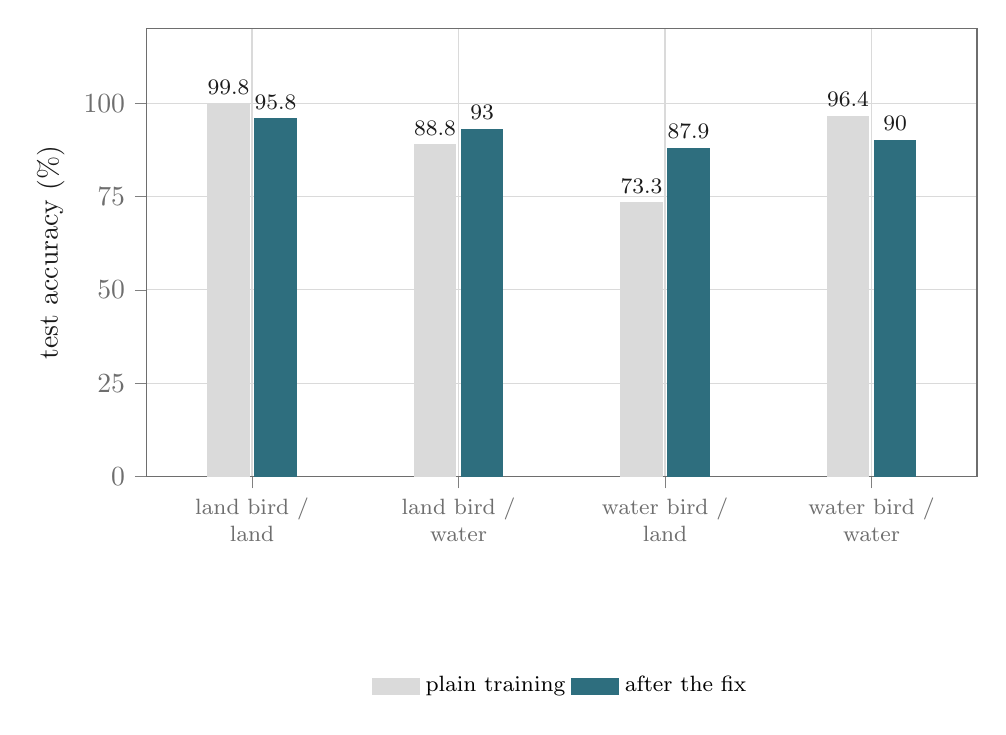
\begin{tikzpicture}
\begin{axis}[slide, width=\linewidth, height=0.60\linewidth,
  ybar, bar width=15pt,
  ymin=0, ymax=120, ytick={0,25,50,75,100},
  ylabel={test accuracy (\%)},
  symbolic x coords={g0,g1,g2,g3}, xtick=data,
  xticklabels={{land bird /\\land},{land bird /\\water},{water bird /\\land},{water bird /\\water}},
  xticklabel style={align=center,font=\figS},
  nodes near coords, nodes near coords style={font=\figS,color=ink},
  every node near coord/.append style={/pgf/number format/fixed,
     /pgf/number format/precision=1},
  enlarge x limits=0.17,
  % -0.24 put the legend on the second line of the two-line tick labels.
  legend style={at={(0.5,-0.42)},anchor=north,legend columns=2,draw=none,
                font=\figS},
]
\addplot[fill=ashe,draw=ashe,area legend] coordinates
  {(g0,99.8)(g1,88.8)(g2,73.3)(g3,96.4)};
\addlegendentry{plain training}
\addplot[fill=teal,draw=teal,area legend] coordinates
  {(g0,95.8)(g1,93.0)(g2,87.9)(g3,90.0)};
\addlegendentry{after the fix}
\end{axis}
\end{tikzpicture}
\par\vskip0.4em
{\footnotesize\color{slate}The groups flatten out. Best-to-worst spread:
\textbf{26.5 points} before, \textbf{7.9} after.}
\end{column}
\begin{column}{0.43\textwidth}
\small
\begin{tabular}{@{}l r r r@{}}
\toprule
\textbf{model} & \textbf{worst} & \textbf{avg} & \textbf{gain}\\
\midrule
plain training & 73.3 & 98.3 & \\
delete 25\%    & 86.4 & 94.7 & \hlt{+13.1}\\
\textbf{delete 50\%} & \hl{87.9} & 94.4 & \hlt{+14.6}\\
delete 75\%    & 87.3 & 92.1 & \hlt{+14.0}\\
\bottomrule
\end{tabular}
\vskip0.9em
{\footnotesize The gain barely moves with the budget, so it needs no
tuning. The average drops about 4 points, the worst group gains 14. \hl{That
trade is the entire point.}}
\vskip0.7em
{\footnotesize\color{slate}Budgets run large because most of each evens up
the bird classes, lopsided at 3682 against 1113.}
\end{column}
\end{columns}
\end{frame}

% ------------------------------------------------------------ 14. RETENTION DEF
\begin{frame}{Phase 2: how we measure whether the fix survived}
{the retention ratio}
\begin{columns}[T,onlytextwidth]
\begin{column}{0.44\textwidth}
\small
$W_p(s)$, $W_e(s)$: worst-group accuracy of the fixed and plain model at the
\emph{same} setting $s$.
\[ D(s)=W_p(s)-W_e(s) \qquad R(s)=\frac{D(s)}{D(0)} \]
$D(0)$ is what the fix bought before compression, $D(s)$ what is left.
\hl{$R$ is the fraction that survived.}
\vskip0.8em
\panel[0.95]{$R\approx 1$: the curves stay apart, the fix
survives.\par\vskip0.3em
$R\approx 0$: they merge. Compression undid the fix, and average accuracy
would never say so.}
\end{column}
\begin{column}{0.52\textwidth}
\centering
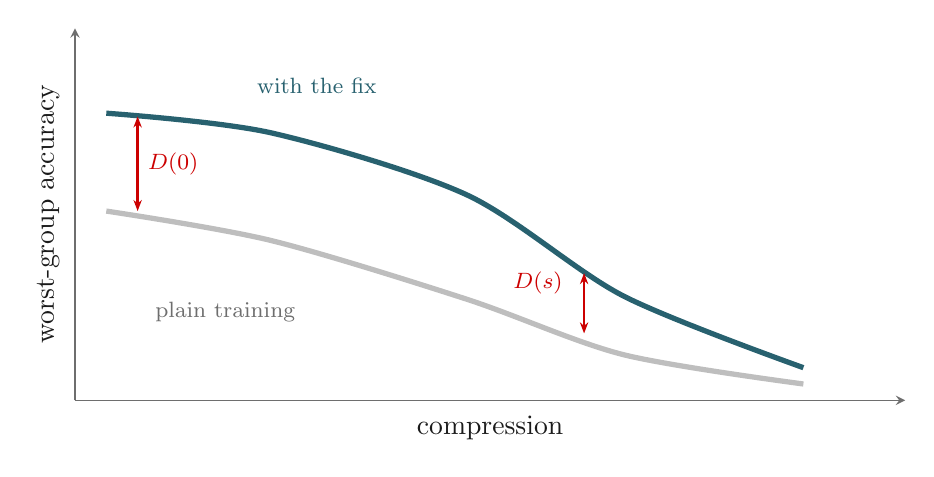
\begin{tikzpicture}
\begin{axis}[slide, width=\linewidth, height=0.52\linewidth,
  xlabel={compression}, ylabel={worst-group accuracy},
  xmin=0, xmax=10.6, ymin=0, ymax=11.4,
  xtick=\empty, ytick=\empty, grid=none, axis lines=left,
]
% The two curves used to be teal and mid grey, close in value and both
% desaturated: from the back they read as one colour. Now dark teal against
% a light grey, the same pairing as the bars on page 15.
\addplot[teal!88!black,line width=1.9pt,smooth] coordinates
  {(0.4,8.8)(2.5,8.2)(5,6.3)(7,3.2)(9.3,1.0)};
% The plain curve runs lower than it used to: the two schematic curves were
% close enough that no label fitted between them without touching one.
\addplot[slate!45,line width=1.9pt,smooth] coordinates
  {(0.4,5.8)(2.5,4.9)(5,3.1)(7,1.4)(9.3,0.5)};
\node[font=\figS,color=teal!88!black,anchor=south west] at (axis cs:2.2,9.1)
  {with the fix};
\node[font=\figS,color=slate,anchor=north west] at (axis cs:0.9,3.3)
  {plain training};
\draw[wolfred,line width=1pt,{Stealth[length=4pt]}-{Stealth[length=4pt]}]
  (axis cs:0.8,8.7) -- (axis cs:0.8,5.8)
  node[midway,right,font=\figS,color=wolfred] {$D(0)$};
\draw[wolfred,line width=1pt,{Stealth[length=4pt]}-{Stealth[length=4pt]}]
  (axis cs:6.5,3.9) -- (axis cs:6.5,2.05);
% Left of its arrow, in the one gap wide enough to hold it.
\node[font=\figS,color=wolfred,anchor=east] at (axis cs:6.35,3.6) {$D(s)$};
\end{axis}
\end{tikzpicture}
\par\vskip0.7em
\callout[0.95]{\textbf{Two things the code refuses to do.} It will not divide
by noise: if $D(0)$ falls below a threshold, $R$ is left undefined and reported
as a null result, because a fabricated ratio is not a finding. And it excludes
collapsed models, because a dead model's retention is meaningless.}
\end{column}
\end{columns}
\end{frame}

% ------------------------------------------------------------ 15. RETENTION RESULT
\begin{frame}{Phase 2: does the fix survive compression?}
{magnitude pruning on the delete 50\% arm, mean of 3 seeds}
\centering
{\small\textbf{Magnitude pruning, step by step}}\par\vskip0.25em
% The table carries the slide on its own now, so it is set a size up and
% spaced out rather than squeezed into a half-width column.
{\fontsize{11}{13.4}\selectfont
\begin{tabular}{@{}l@{\hspace{3.2em}}r@{\hspace{3.2em}}r@{\hspace{3.2em}}r@{}}
\toprule
\textbf{weights removed} & \textbf{plain} & \textbf{fixed} & \textbf{R}\\
\midrule
none & 73.3 & 87.9 & 1.00\\
30\% & 58.4 & 81.9 & \hlt{$+1.64$}\\
50\% & 23.7 & 53.0 & \hlt{$+2.04$}\\
70\% & 13.7 & 13.4 & \hl{$-0.15$}\\
\bottomrule
\end{tabular}}
\par\vskip0.4em
{\footnotesize\color{slate}Worst-group accuracy without and with the fix, and
$R$, the share of the original gain still standing.}
\par\vskip0.55em
\begin{columns}[T,onlytextwidth]
\begin{column}{0.47\textwidth}
\panel[0.95]{\textbf{Read the 70\% row carefully.} At 70\% \emph{neither}
model works, both near 13\%. $R$ is a ratio of two gaps and both are gone, so
a zero means \hl{the question no longer applies}, not ``the fix was
destroyed''.}
\end{column}
\begin{column}{0.47\textwidth}
\callout[0.95]{\textbf{\color{wolfred}The answer.} If compression leaves a
working model, the fix is still there 95\% of the time, across \emph{all
four} families. If the model is already dead, $R$ is noise. No middle ground,
no family behaving specially.}
\end{column}
\end{columns}
\end{frame}

% ------------------------------------------------------------ 16. VS PAPER
\begin{frame}{Compared with the published result, and an honest limitation}
{the same deletion rule on a different backbone, and what it does at large
budgets}
\begin{columns}[T,onlytextwidth]
\begin{column}{0.43\textwidth}
\small
\begin{tabular}{@{}l r r@{}}
\toprule
 & \textbf{plain} & \textbf{with fix}\\
\midrule
the paper, ResNet-50   & 74.8 & \textbf{90.9}\\
this project, ViT-S/16 & 73.3 & \textbf{87.9}\\
\bottomrule
\end{tabular}
\vskip0.4em
{\footnotesize Worst-group accuracy at the \textbf{delete 50\%} budget,
where 4795 training images become 1170. Our plain baseline is within 1.5
points of it.}
\vskip0.6em
\panel[0.95]{\textbf{Where the gap comes from.} The ranking is informative
only while the model has not yet learned the training set. The paper trains
from scratch for 100 epochs; ours is pretrained and reaches \hl{97.9\% in two
passes}.}
\end{column}
\begin{column}{0.53\textwidth}
\centering
{\footnotesize
\begin{tabular}{@{}l r r@{}}
\toprule
\textbf{images we delete} & \textbf{genuinely hard} &
\textbf{already easy}\\
\midrule
delete 25\% & 1080 & \hl{2017 (65\%)}\\
delete 50\% & 1344 & \hl{2281 (63\%)}\\
delete 75\% & 1479 & \hl{2676 (64\%)}\\
\bottomrule
\end{tabular}}
\par\vskip0.2em
{\fontsize{8}{9.6}\selectfont\color{slate}\emph{already easy}: above 99.3\%
on the true label after one epoch.}
\par\vskip0.45em
\callout[0.96]{Two thirds of what we delete, the model already gets almost
perfectly: at these budgets the pool of hard images runs out first. What is
left is closer to \emph{shrink and balance the training set}, itself a known
way to help weak groups. \hl{This follows from the budget sizes, not from our
implementation.}}
\end{column}
\end{columns}
\vskip0.3em
{\fontsize{8}{10}\selectfont\color{slate}Varun Mulchandani and Jung-Eun Kim.
\emph{Severing Spurious Correlations with Data Pruning}. ICLR 2025,
arXiv:2503.18258. We reproduce the identifiable-setting rule of section 6.3.}
\end{frame}

% ------------------------------------------------------------ 17. CHALLENGES
\begin{frame}{Main challenges}
{two decisions that shaped the method, and the tests that check them}
\begin{columns}[T,onlytextwidth]
\begin{column}{0.315\textwidth}
{\small\textbf{\color{wolfred}Scientific}}\par\vskip0.4em
{\footnotesize
\textbf{$R$ is read one compression level at a time.} Magnitude gives
$+2.04$ at 50\% and $-0.15$ at 70\%; the average of the two describes
neither, and pooling levels suggested a per-family effect the per-level
numbers do not support.
\vskip0.5em
\textbf{The deletion rule has to be group-aware.} Ranking on difficulty
alone removes the very images the fix protects, so only shortcut-aligned
ones are deleted.}
\end{column}
\begin{column}{0.315\textwidth}
{\small\textbf{\color{wolfred}Engineering}}\par\vskip0.4em
{\footnotesize
\textbf{Scoring shares a code path with saving.} The early-epoch scoring run
reaches the same ``save if best so far'' branch, so a truncated run could
overwrite a finished checkpoint. V13 checks that it cannot.
\vskip0.5em
\textbf{Run counts come from the files, not the logs.} A step can log success
and still fail while writing, so the logs overcounted.}
\end{column}
\begin{column}{0.315\textwidth}
{\small\textbf{\color{wolfred}What the tests check}}\par\vskip0.4em
{\footnotesize 64 Python gates and 15 shell assertions, one claim each.}
\vskip0.35em
{\fontsize{9}{10.8}\selectfont
\begin{tabular}{@{}l l@{}}
\toprule
\textbf{gate} & \textbf{claims}\\
\midrule
V4  & magnitude zeroes exactly $k$\\
V5  & masking equals real deletion\\
V7b & the baseline has not collapsed\\
V8  & \texttt{apply} never mutates input\\
V13 & a truncated run saves no model\\
V17 & no counter-shortcut deletions\\
V18 & the kept classes end up equal\\
\bottomrule
\end{tabular}}
\end{column}
\end{columns}
\end{frame}

% ------------------------------------------------------------ 18. CONTRIBUTIONS
\begin{frame}[t]{Each member's contribution}
{who built which part of the pipeline, and what it took}
\vskip0.1em
\begin{columns}[T,onlytextwidth]
\begin{column}{0.315\textwidth}
\colorbox{wolfred}{\makebox[\textwidth][l]{\rule{0pt}{2.5ex}%
  \color{white}\footnotesize\textbf{~Shreyas Visweshwaran}~~sviswes%
  \rule[-1.2ex]{0pt}{0pt}}}
\vskip0.5em
{\footnotesize
\textbf{Compression methods.} All four families behind one \texttt{apply}
contract: magnitude pruning, attention-head and FFN-neuron removal, and
quantization at two granularities, head removal exact, not approximate.
\vskip0.32em
\textbf{The frozen scope.} The 21,233,664 weights every method may touch,
fixed once so one sparsity axis means the same thing in all four families.
\vskip0.32em
\textbf{Phase 1 sweep.} The 29-setting driver, its pristine-source check, a
resume key separating arm, seed and checkpoint, and 87 measurements.}
\end{column}
\begin{column}{0.315\textwidth}
\colorbox{wolfred}{\makebox[\textwidth][l]{\rule{0pt}{2.5ex}%
  \color{white}\footnotesize\textbf{~Swasti Sadanand}~~ssadana%
  \rule[-1.2ex]{0pt}{0pt}}}
\vskip0.5em
{\footnotesize
\textbf{Phase 2 data-pruning fix.} Difficulty scored after one epoch, both
pruning variants built, and the evidence that the group-blind one deletes
the very images the fix protects.
\vskip0.32em
\textbf{Retention ratio.} Defining $R$, the gate that leaves it undefined
when $D(0)$ is within noise, and the usability buckets behind the 95\%
headline.
\vskip0.32em
\textbf{Comparison to the paper.} The delete 50\% result reproduced on a
different backbone, with the 3-point shortfall traced to a ranking that
flattens on a pretrained model.}
\end{column}
\begin{column}{0.315\textwidth}
\colorbox{wolfred}{\makebox[\textwidth][l]{\rule{0pt}{2.5ex}%
  \color{white}\footnotesize\textbf{~Anusha Upadhyay}~~aupadhy6%
  \rule[-1.2ex]{0pt}{0pt}}}
\vskip0.5em
{\footnotesize
\textbf{Metrics and collapse detection.} Group indexing, per-group and
adjusted-average accuracy, and the \texttt{pred\_mean} gate that stops a
model predicting one class everywhere from reading as fair.
\vskip0.32em
\textbf{Test suite.} 64 Python gates and 15 shell assertions, among them the
proofs that masked head removal equals real deletion and that no method
mutates its input.
\vskip0.32em
\textbf{Figures.} The three figure families, the summary tables, and the
hollow-marker convention that keeps collapsed settings visible.}
\end{column}
\end{columns}
\end{frame}

% ------------------------------------------------------------ 19. TAKEAWAYS
\begin{frame}[t]{What we would want remembered}
{five results, and three ways this project departs from the paper}
\vskip0.1em
\begin{columns}[T,onlytextwidth]
\begin{column}{0.48\textwidth}
\small
\begin{enumerate}\setlength{\itemsep}{0.5em}
\item \textbf{Average accuracy hides group damage.} 0.5 points against 14.9
from the same operation, a 29-fold difference.
\item \textbf{Where you cut matters more than how much.} 6 heads of 72 is
2.8\% of the scope and costs 18.2 points. 30\% magnitude pruning costs 14.9.
\item \textbf{A collapsed model looks fair.} One class for every image, no
gap at all, and still a 76.8\% adjusted average.
\item \textbf{The fix works, and survives until compression breaks the model
outright.} Worst group 73.3 to 87.9, still there 95\% of the time wherever
the model is usable.
\end{enumerate}
\end{column}
\begin{column}{0.48\textwidth}
\small
\begin{enumerate}\setlength{\itemsep}{0.5em}\setcounter{enumi}{4}
\item \textbf{$R$ is read one compression level at a time.} Pooled across
levels it suggested a per-family effect the per-level numbers do not support.
\item \textbf{A different backbone.} ResNet-50 from scratch for 100 epochs
in the paper; a pretrained ViT-S/16 fine-tuned for 10 here, and the rule
still adds 14.6 worst-group points.
\item \textbf{We carry the fix past training.} The paper stops at the
trained model; we compress it 29 ways, never retraining after, and read with
$R$ what is left.
\item \textbf{We looked at what the rule deletes.} At these budgets two
thirds of the deleted images are ones the model already gets right.
\end{enumerate}
\end{column}
\end{columns}
\end{frame}

% ------------------------------------------------------------ 20. CLOSING
{%
\setbeamertemplate{footline}{}
\begin{frame}[plain]
\begin{tikzpicture}[remember picture,overlay]
  \shade[shading angle=25, top color=wolfred, bottom color=deepred]
    (current page.south west) rectangle (current page.north east);
  \shade[shading angle=115, top color=deepred, bottom color=midred,
         opacity=0.38]
    (current page.south west) rectangle (current page.north east);

  % No corner badge here: the two codes below are the whole point of the slide.
  \node[anchor=south] at ($(current page.center)+(0,2.75)$)
    {\color{white}\rule{2.2em}{2.4pt}};

  \node[anchor=south,text width=0.82\paperwidth,align=center]
    at ($(current page.center)+(0,0.55)$) {%
    \color{white}\fontsize{26}{30}\selectfont\bfseries Thank\,\,you\par
    \vskip0.5em
    {\fontsize{11}{14}\selectfont\mdseries
    Anusha Upadhyay\quad Shreyas Visweshwaran\quad Swasti Sadanand}
  };

  % The two codes, side by side. White backing gives each its quiet zone
  % against the gradient, which a scanner needs.
  \node[anchor=north] at ($(current page.center)+(0,-0.15)$) {%
    \begin{tabular}{@{}c@{\hspace{3em}}c@{}}
      \colorbox{white}{\usebox{\qrreport}} &
      \colorbox{white}{\usebox{\qrrepo}}\\[0.45em]
      {\color{white}\footnotesize the explainer} &
      {\color{white}\footnotesize the code}\\
    \end{tabular}};
\end{tikzpicture}
\end{frame}
}

\end{document}
